% !TEX root = main.tex

\section{并发---死锁与饥饿}
\subsubsection{死锁}
死锁(deadlock):一个进程集合中的每个进程都在等待只能由该集合中的其他一个进程才能引发的事件(释放占有资源/进行某项操作)
\begin{figure}[H]
    \centering
    \begin{tabular}{c}
    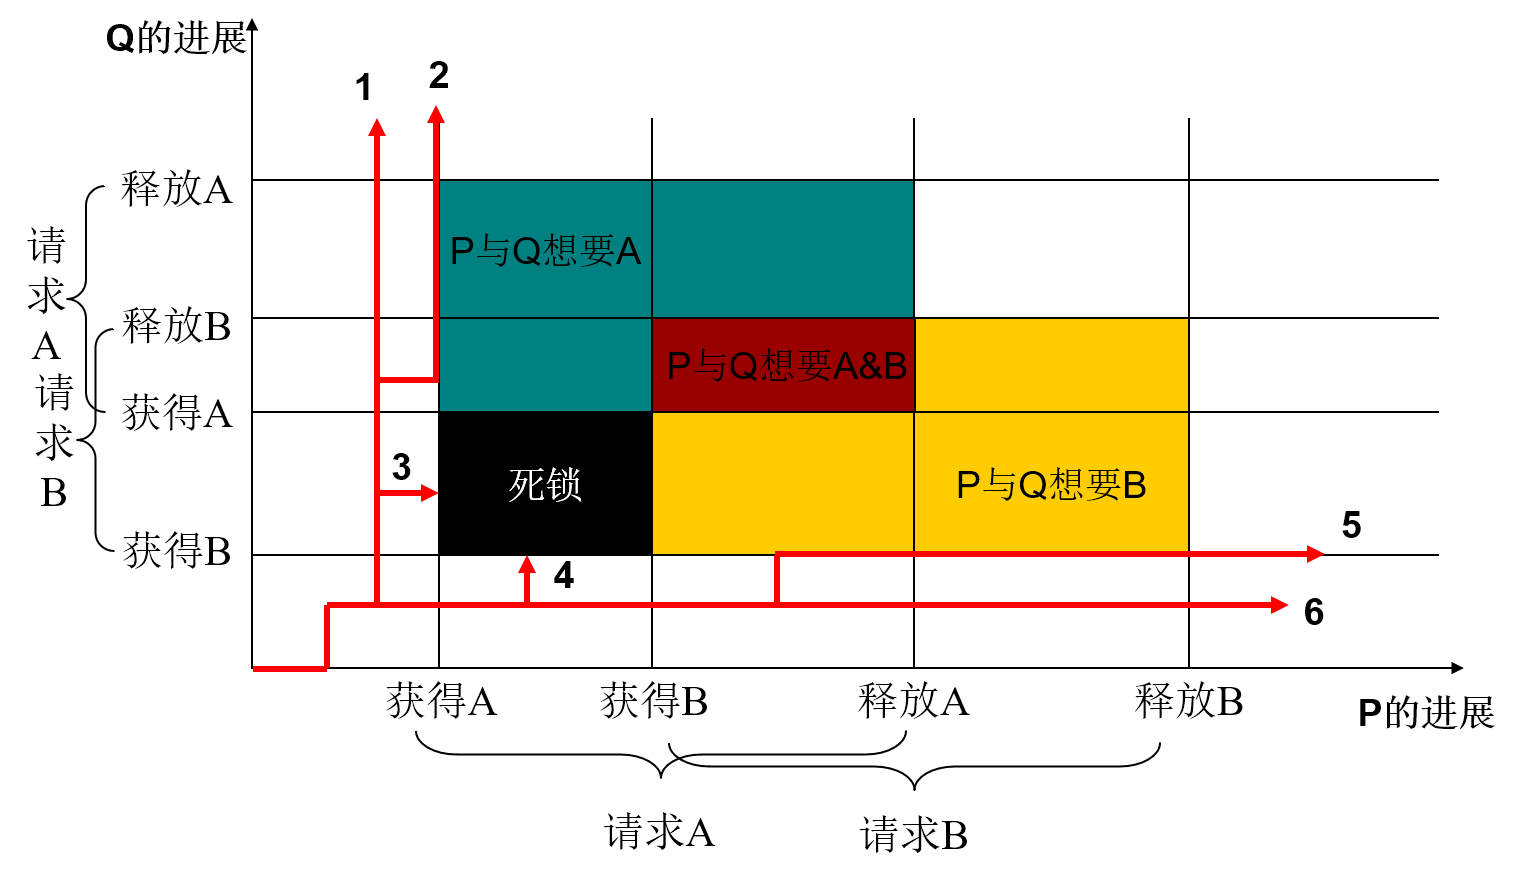
\includegraphics[width=0.8\linewidth]{fig/deadlock.png}\\
    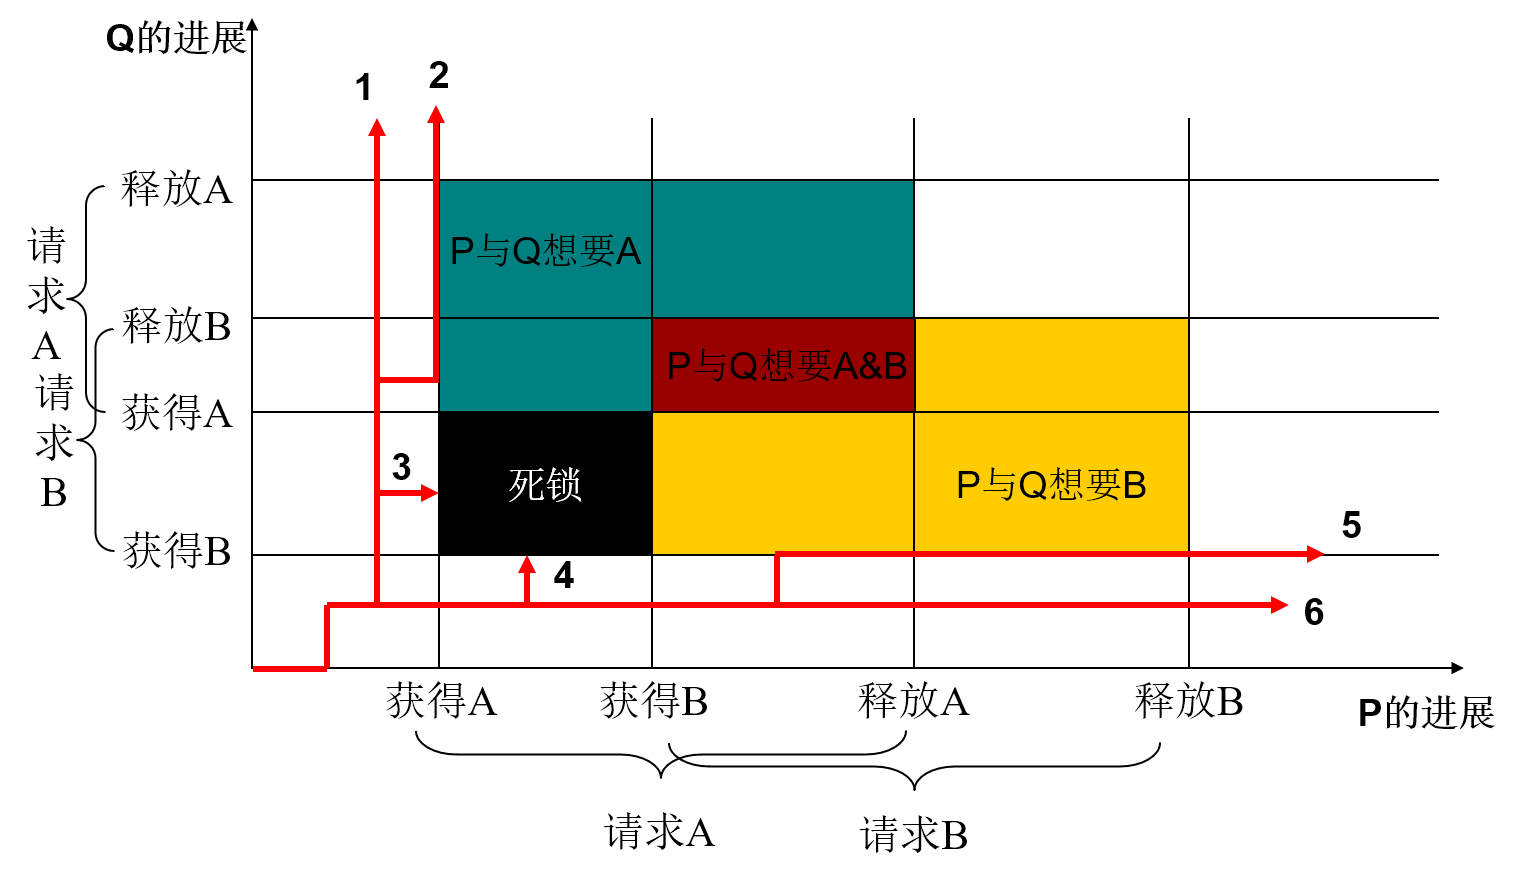
\includegraphics[width=0.8\linewidth]{fig/deadlock.png}
    \end{tabular}
    \caption*{联合进程图,上图死锁,下图无死锁}
\end{figure}

\begin{center}
\begin{tabular}{|l|l|l|p{10em}|l|}
\hline
\multicolumn{1}{|p{3.065em}|}{原则} & \multicolumn{1}{p{6em}|}{资源分配策略} & \multicolumn{1}{p{10em}|}{不同的方案} & 主要优点  & \multicolumn{1}{p{10em}|}{主要缺点} \bigstrut\\
\hline
\multicolumn{1}{|l|}{\multirow{6}[6]{*}{预防}} & \multicolumn{1}{l|}{\multirow{6}[6]{*}{保守,预提交(undercommits)资源}} & \multicolumn{1}{l|}{\multirow{3}[2]{*}{一次性请求所有资源}} & \tabitem对执行单一突发行为的进程有效 & \multicolumn{1}{p{10em}|}{\tabitem低效} \bigstrut[t]\\
      &       &       & \tabitem不需抢占 & \multicolumn{1}{p{10em}|}{\tabitem延时进程的初始化} \\
      &       &       & \multicolumn{1}{r|}{} & \multicolumn{1}{p{10em}|}{\tabitem进程必须知道未来的资源请求} \bigstrut[b]\\
\cline{3-5}      &       & \multicolumn{1}{p{10em}|}{抢占} & \tabitem便于用于状态易保存和恢复的资源 & \multicolumn{1}{p{10em}|}{\tabitem过多的不必要抢占} \bigstrut\\
\cline{3-5}      &       & \multicolumn{1}{l|}{\multirow{2}[2]{*}{资源排序}} & \tabitem通过编译时检测可实施 & \multicolumn{1}{l|}{\multirow{2}[2]{*}{\tabitem不允许增加资源请求}} \bigstrut[t]\\
      &       &       & \tabitem由于问题已在系统设计时解决,不需运行时再计算 &  \bigstrut[b]\\
\hline
\multicolumn{1}{|l|}{\multirow{2}[2]{*}{避免}} & \multicolumn{1}{l|}{\multirow{2}[2]{*}{位于检测和预防中间}} & \multicolumn{1}{l|}{\multirow{2}[2]{*}{操纵以发现至少一条安全路径}} & \multirow{2}[2]{*}{\tabitem不需抢占} & \multicolumn{1}{p{10em}|}{\tabitem OS必须知道未来的资源请求} \bigstrut[t]\\
      &       &       & \multicolumn{1}{l|}{} & \multicolumn{1}{p{10em}|}{\tabitem进程可能被长期阻塞} \bigstrut[b]\\
\hline
\multicolumn{1}{|l|}{\multirow{2}[2]{*}{检测}} & \multicolumn{1}{l|}{\multirow{2}[2]{*}{非常自由;尽可能地准许请求的资源}} & \multicolumn{1}{l|}{\multirow{2}[2]{*}{周期性地调用以测试死锁}} & \tabitem不会延时进程的初始化 & \multicolumn{1}{l|}{\multirow{2}[2]{*}{\tabitem丢失固有抢占}} \bigstrut[t]\\
      &       &       & \tabitem易于在线处理 &  \bigstrut[b]\\
\hline
\end{tabular}%
\end{center}

死锁定理:资源分配图中存在环路是存在死锁的充分必要条件
\begin{figure}[H]
    \centering
    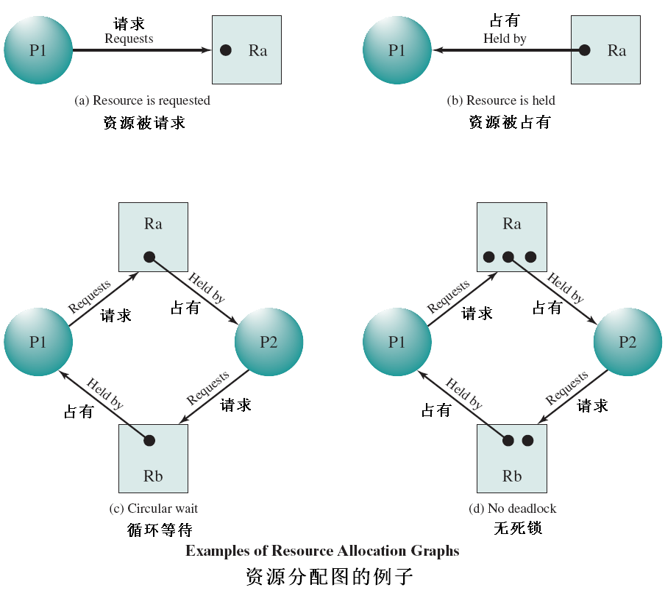
\includegraphics[width=0.6\linewidth]{fig/resource_graph.png}
\end{figure}

死锁的充分必要条件
\begin{itemize}
    \item 互斥
    \item 占有且等待
    \item 不可抢占
    \item 循环等待
\end{itemize}

\subsection{死锁预防}
破坏互斥条件:允许多个进程同时使用资源,但不适用于绝大多数资源

适用条件
\begin{itemize}
\item 资源的固有特性允许多个进程同时使用(如文件允许多个进程同时读)
\item 借助特殊技术允许多个进程同时使用(如打印机借助Spooling技术)
\end{itemize}

破坏占有且等待条件:禁止已拥有资源的进程再申请其他资源,如要求所有进程在开始时一次性地申请在整个运行过程所需的全部资源;或申请资源时要先释放其占有资源后,再一次性申请所需全部资源
\begin{itemize}
    \item 优点:简单、易于实现、安全
    \item 缺点:进程延迟运行,资源严重浪费
\end{itemize}

破坏不可剥夺条件:一个已经占有了某些资源的进程,当它再提出新的资源请求而不能立即得到满足时,必须释放它已经占有的所有资源,待以后需要时再重新申请;OS可以剥夺一个进程占有的资源,分配给其他进程

适用条件:资源的状态可以很容易地保存和恢复(如CPU)
缺点:实现复杂、代价大,反复申请/释放资源、系统开销大、降低系统吞吐量

破坏环路等待条件方法
\begin{itemize}
    \item 要求每个进程任何时刻只能占有一个资源,如果要申请第二个则必须先释放第一个(不现实)
    \item 对所有资源按类型进行线性排队,进程申请资源必须严格按资源序号递增的顺序(可避免循环等待)
\end{itemize}

缺点
\begin{itemize}
    \item 很难找到令每个人都满意的编号次序,类型序号的安排只能考虑一般作业的情况, 限制了用户简单、自主地编程
    \item 易造成资源的浪费(会不必要地拒绝对资源的访问)
    \item 可能低效(会使进程的执行速度变慢)
\end{itemize}

\subsection{死锁避免}
进程启动拒绝

进程分配拒绝:银行家算法(Dijkstra)
% 具体图示
\begin{itemize}
    \item 只要系统处于安全状态,必定不会进入死锁状态
    \item 不安全状态不一定是死锁状态,但不能保证不会进入死锁状态
    \item 如果一个新进程的资源请求会导致不安全状态,则拒绝启动这个进程
\end{itemize}

优点
\begin{itemize}
    \item 比死锁预防限制少
    \item 无须死锁检测中的资源剥夺和进程重启
\end{itemize}
缺点
\begin{itemize}
    \item 必须事先声明每个进程请求最大资源
    \item 进程必须无关,没有同步要求
    \item 分配的资源数目是固定的
    \item 占有资源时进程不能退出
\end{itemize}

\subsection{死锁检测}
检测方法:
\begin{itemize}
    \item 单个资源实例:检测资源分配图中是否存在环路(依据——死锁定理)
    \item 多个资源实例:类似银行家算法的安全检查
\end{itemize}

恢复:
\begin{itemize}
    \item 剥夺法:连续剥夺资源指导不存在死锁
    \item 回退法:将每个死锁进程回滚到前面定义的某些检查点(checkpoint),并重启所有进程(死锁可能重现)
    \item 杀死进程法
\end{itemize}

\subsubsection{饥饿}
饥饿:一组进程中,某个或某些进程\textbf{无限等待}该组进程中其他进程所占用的资源